\subsection{RAP-MUSIC}
Rekursiivisesti sovelletun ja projisoidun MUSIC (recursively applied and projected MUSIC, RAP-MUSIC) \citep{Mosher1999SourceMUSIC} on MUSIC-algoritmin iteratiivinen versio, jossa löydetyn lähteen topografia projisoidaan pois signaaliavaruudesta ennen seuraavan lähteen paikantamista. Tämän jälkeen seuraava lähde etsitään muunnetun signaaliavaruuden paikannusfunktion maksimina. RAP-MUSICin etuna on, että se löytää lähdepisteet yksi kerrallaan eikä kaikkia lähdepisteitä kerralla tavallisen MUSIC-algoritmin tapaan \citep{Makela2018TruncatedLocalization}.

%RAP-MUSIC löytää hyvin korreloituneita lähteitä tavallista MUSICia paremmin

Tarkastellaan ensin kiinteän orientaation tapausta. RAP-MUSIC alkaa tavallisen MUSIC-algoritmin tapaan löytäen ensimmäisen maksimipisteen estimaatin \textbf{\^p}, jolla on topografia \textbf{l(\^p)}. Iteraatiokierrosta \textit{k}+1 varten muodostamme projektio-operaattorin, joka projisoi löydettyjen lähdepisteiden $\mathbf{p}_1,...,\mathbf{p}_{k}$ topografiat pois signaaliavaruudesta:

\begin{equation}
    \mathbf{Q}_k = \mathbf{I}-\mathbf{B}_k\mathbf{B}_k^\dagger,
\end{equation}
jossa $\mathbf{B}_k = [\mathbf{l(p}_1),...,\mathbf{l(p}_{k})]$ sisältää löydettyjen lähteiden topografiat. Muunnettu signaaliavaruus on täten $\mathbf{Q}_k\mathbf{U}(:,1:\Tilde{n})$, jossa $\Tilde{n} \geq n$ on approksimoitujen lähteiden määrä. Muodostetaan muunnetun signaaliavaruuden virittäjämatriisista $\mathbf{Q}_k\mathbf{U}(:,1:\Tilde{n})$ singulaariarvohajotelma:

\begin{equation}
    \mathbf{Q}_k\mathbf{U}(:,1:\Tilde{n}) = \mathbf{U}_k\mathbf{D}_k\mathbf{V}_k^T
    \label{eq:rap}
\end{equation}
ja sen avulla projektio muunnettuun signaaliavaruuteen:
\begin{equation}
    \mathbf{P}_k = \mathbf{Q}_k\mathbf{U}(:,1:\Tilde{n})(\mathbf{Q}_k\mathbf{U}(:,1:\Tilde{n}))^{\dagger} = \mathbf{U}_k(1:\Tilde{n})\mathbf{U}_k(1:\Tilde{n})^T
\end{equation}

Kiinteän orientaation paikannusfunktio on
\begin{equation}
    \mathbf{\mu_k(p)} = \frac{||\mathbf{P}_k\mathbf{Q}_k\mathbf{l(p)}||^2}{||\mathbf{Q}_k\mathbf{l(p)}||^2}
    \begin{cases}
    =1\text{, jos $\mathbf{p}$ on lähdepiste}\\
    <1\text{, jos $\mathbf{p}$ ei ole lähdepiste}
     \end{cases}
\end{equation}
Vapaan orientaation paikannusfunktio saadaan edellisen kappaleen mukaisesti:
\begin{equation}
    \mathbf{\mu_k(p)} = \max_{||\eta||=1} \frac{||\mathbf{P}_k\mathbf{Q}_k\mathbf{L(p)\eta}||^2}{||\mathbf{Q}_k\mathbf{L(p)\eta}||^2}
    \begin{cases}
    =1\text{, jos $\mathbf{p}$ on lähdepiste}\\
    <1\text{, jos $\mathbf{p}$ ei ole lähdepiste}
     \end{cases}
\end{equation}

RAP-MUSIC:n paikannusfunktio saattaa löytää vääriä lähdepisteitä jo löydettyjen lähteiden läheltä, joka johtuu siitä, ettei algoritmi pysty täysin poistamaan topografiaa löydettyjen dipolien paikalta. RAP-dilemmaa havaitaan varsinkin kohinattomalla ja valkoisen kohinan datalla. RAP-dilemman vuoksi singulaariarvoissa ei havaita selkeää pudotusta, joka voi johtaa väärään lähteiden lukumäärän arvioimiseen. \citep{Makela2018TruncatedLocalization}

\begin{figure}[hb]
    \centering
    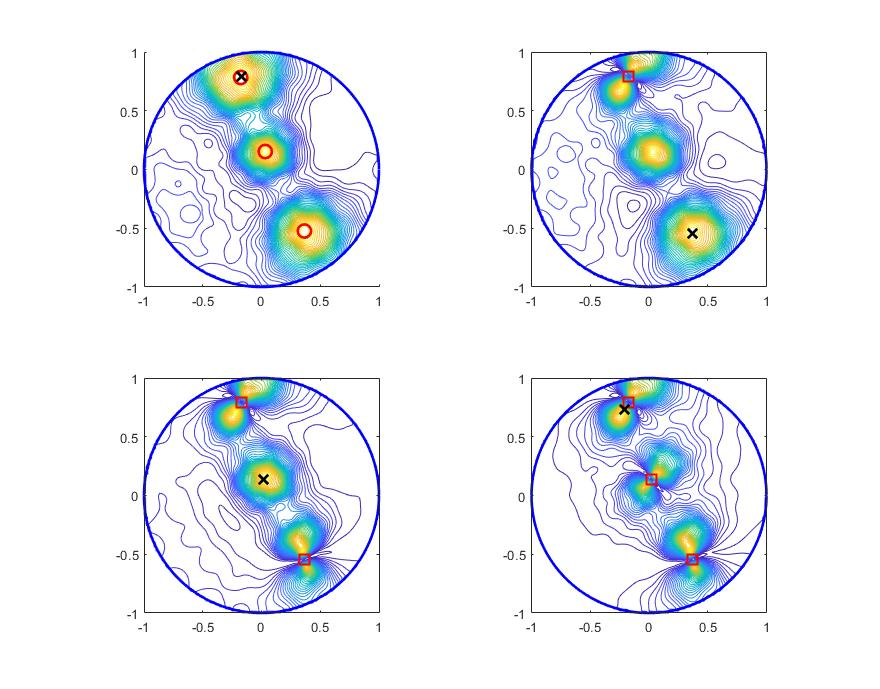
\includegraphics[width=\textwidth]{rapdilemma.jpg}
    \caption{RAP-dilemmaa havainnoillistava kuva. Musta rasti kuvaa iteraatiokierroksella löydettyä paikannusfunktion maksimia ja punaiset neliöt löydettyjä lähteitä. Kuvista huomataan suuret paikannusfuntion saamat arvot jo löydettyjen lähteiden ympäriltä.}
    \label{fig:dilemma}
\end{figure}